
%(BEGIN_QUESTION)
% Copyright 2009, Tony R. Kuphaldt, released under the Creative Commons Attribution License (v 1.0)
% This means you may do almost anything with this work of mine, so long as you give me proper credit

Suppose this Foxboro model 13 DP transmitter has a calibrated range of 0 to 125 inches water column and an instrument air supply pressure of 20 PSI:

$$\includegraphics[width=15.5cm]{i03936x01.eps}$$

Identify which way the range wheel would have to be moved in order to re-calibrate the transmitter to a new range of 0 to 180 inches water column (from 0 to 125 "W.C.), explaining your reasoning.

\vskip 10pt

Identify which way the zero screw would have to be turned in order to re-calibrate the transmitter to a new range of 15 to 140 inches water column (from 0 to 125 "W.C.), explaining your reasoning.

\vskip 20pt \vbox{\hrule \hbox{\strut \vrule{} {\bf Suggestions for Socratic discussion} \vrule} \hrule}

\begin{itemize}
\item{} Explain why it is important we know whether this mechanism is motion- or force-balance to be able to correctly determine the effects these changes will have on calibration.
\item{} What would happen if the capsule were to develop a leak?
\item{} What would happen if the flexure connecting the tops of the force and range bars were to break in half, leaving those two bars disconnected from each other?
\item{} What would happen if the air supply pressure were to increase from 20 PSI to 22 PSI?
\item{} What would happen if the air supply pressure were to decrease from 20 PSI to 18 PSI?
\end{itemize}

\underbar{file i03936}
%(END_QUESTION)





%(BEGIN_ANSWER)

Move the range wheel {\it up} in order to re-calibrate from 0-125 "W.C. to 0-180 "W.C.

\vskip 10pt

Turn the zero screw for {\it less} tension against the range bar (less force pulling the bottom of the range bar to the right) in order to re-calibrate from 0-125 "W.C. to 15-140 "W.C.

%(END_ANSWER)





%(BEGIN_NOTES)

The range wheel would have to be moved {\it up} to re-calibrate the transmitter from 0-125 "W.C. to 0-180 "W.C., because this represents a greater range of applied pressure to the sensing diaphragm, and therefore a greater range of force at the top of the force bar.  In order for the same range of 3-15 PSI at the bellows to counter-act (balance) the greater force at the force bar, the bellows must be given more of a mechanical advantage (i.e. more force multiplication).

\vskip 10pt

The zero screw would have to be turned such that the zero spring pulls with less force against the bottom of the range bar.  The new range of 15-140 "W.C. represents a zero-shift in pressure applied to the sensing diaphragm.  Thus, we are seeing more force on the ``high'' side of the diaphragm than before (with the old range of 0-125 "W.C.).  More diaphragm force means more bellows force against the range bar than before, all other factors being equal.  We want the bellows force to be the same (3-15 PSI), however, even with this new (greater) process fluid force.  Therefore, the zero spring needs to relax its tension against the range bar.

\vskip 10pt

The 20 PSI supply air pressure is extraneous information, included for the purpose of challenging students to identify whether or not information is relevant to solving a particular problem.

%INDEX% Calibration, pneumatic instrument: zero and span adjustments

%(END_NOTES)


